%Dokumentklasse Festlegen
\documentclass[paper = a4, ngerman]{scrartcl}

	%ngerman fur Umlaute, Anf"hrungszeichen, etc.%
	\usepackage[ngerman]{babel, varioref}

	%siunitx fur SI-Einheitesnsystem%
	\usepackage{siunitx}
	\sisetup{
	    locale=DE,
	    separate-uncertainty=true,
    	per-mode=fraction
	}

	%graphicx fur Bildeinbindung%
	\usepackage{graphicx}

	%enthaelt eqnref{}-Operator
	\usepackage{amsmath}

	%Links innerhalb und ausserhalb des Dokuments
	\usepackage{hyperref}

	%Formatiert urls
	\usepackage{url}

	% Seitenlayout ändern mit Fancy
	\usepackage{fancyhdr}	% Paket zum bequemeren Verändern des Seitenlayouts

		% Tabellen ändern:
			\renewcommand{\thetable}{\arabic{section}.\arabic{table}} % figures bekommen die richtige Nummerierung: x.y
			\makeatletter \@addtoreset{table}{section} \makeatother      % nach jeder section wird neu gezählt

		% Kapitelüberschriften in der Kopfzeile:
			\renewcommand*{\sectionmark}[1]{\markboth{}{\thesection\ #1}}
			%\renewcommand*{\subsectionmark}[1]{\markboth{}{\thesubsection\ #1}}
			\renewcommand*{\subsectionmark}[1]{\markboth{}{}} % keine Unterüberschriften in der Kopfzeile
			\renewcommand{\plainheadrulewidth}{0.4pt}
		
		% Seitennummern rechts in der Kopfzeile:
			\lhead[\fancyplain{\thepage}{\thepage}]{\fancyplain{}{\rightmark}}
			\rhead[\fancyplain{}{\leftmark}]{\fancyplain{\thepage}{\thepage}}
		
		%Fußzeilen bleiben leer
			\lfoot{}
			\cfoot{}
			\rfoot{}

	%Texteinzug vor Absatz entfernen%
	\parindent 0pt

	%Titelseiten Parameter
	\title{V406 - Beugung am Spalt}
	\date{27. Oktober 2012}
	\author{Kevin Heinicke und Markus Stabrin}

\begin{document}

	%\maketitle

	% ANFANG Titelseite %
	\vspace*{3cm}

	\begin{center}
		\large
		TU Dortmund
	\end{center}

	\begin{center}
		\Huge
		V406 - Beugung am Spalt
	\end{center}

	\vspace{6cm}
	\begin{center}
		\begin{minipage}[b]{8cm}
			\Large
			Markus Stabrin \\
			\normalsize
			markus.stabrin@tu-dortmund.de \\

			\Large
			Kevin Heinicke\\
			\normalsize
			kevin.heinicke@tu-dortmund.de \\
			\\
			\\

			Versuchsdatum: 23. Oktober 2012 \\
			\\
			Abgabedatum: 30. Oktober 2012
		\end{minipage}
	\end{center}

	% ENDE Titelseite %

	\newpage

	\section{Einleitung}
	In diesem Versuch wurde die Ablenkung von Elektronen in elektrischen und magnetischen Feldern untersucht.
	Die theoretischen Grundlagen sollten zun"achst mit Messdaten "uber\-pr"uft werden.
	Schlie"slich wurden die Erkenntnisse genutzt, um ein einfaches Oszilloskop zu realisieren und die Feldst"arke des Erdmagnetfeldes zu messen.

\section{Funktionsweise und Theoretische Grundlagen}
	Im Folgenden werden aus den wirkenden Kr"aften die zu "uberpr"ufenden Zusammenh"ange hergeleitet.

	\subsection{Elektrische Kraft}
		Im ersten Versuch betrachtet man ausschlie"slich die elektrische Kraft $\vec{F}_\mathrm{el}$, die auf eine Ladung $q$ im elektrischen Feld $\vec{E}$ wirkt.
		In unserem Versuchsaufbau durchl"auft ein Elektronenstrahl eine Anordnung aus Plattenkondesatoren,
		in denen das elektrische Feld "uberall n"aherungsweise senkrecht auf den Kondensatorplatten steht.

		Die Platten haben die L"ange $p$ und seien im Abstand $d$ angebracht. An ihnen liegt eine Spannung $U_\mathrm{d}$ an.
		Die Ladung der Elektronen betr"agt $e$, ihre Masse $m_e$.

		Die Geschwindigkeit $\vec{v}$ der Teilchen l"asst sich in die Komponenten $v_\mathrm{y}$ und $v_\mathrm{z}$ zerlegen,
		die parallel bzw. orthogonal zum elektrischen Feld $\vec{E}$ stehen.

		Es kann damit eine Aussage "uber den Winkel $\theta$ zwischen $v_\mathrm{y}$ und $v_\mathrm{z}$ getroffen werden:

		\begin{eqnarray}
			\theta & = & \frac{e}{m_e} \frac{U_\mathrm{d}}{d} \frac{p}{v_\mathrm{z}^2}
			\label{theta}
		\end{eqnarray}

		\begin{figure}[h]
			\centering
			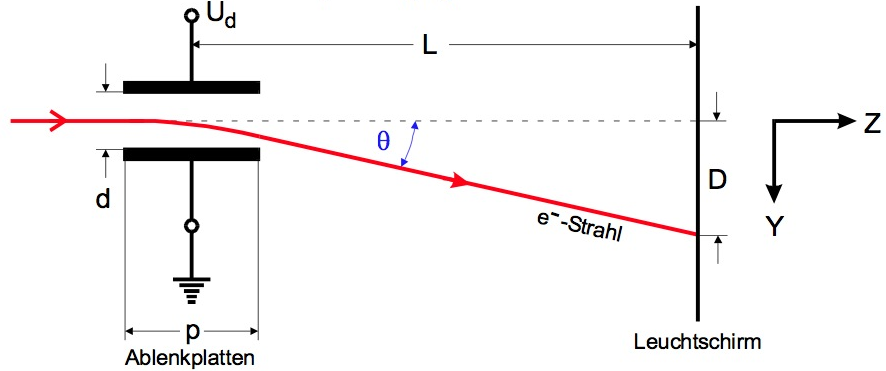
\includegraphics[width = 14cm]{img/ablenkung.png}
			\caption{Strahlablenkung durch einen Plattenkondensator}
			\label{ablenkung}
		\end{figure}

		Unter Ber"ucksichtigung der Beschleunigungsspannung $U_\mathrm{B}$ (siehe \ref{wehnelt}) gilt f"ur die Verschiebung $D$ im Abstand $L$ und parallel zu $\vec{E}$:

		\begin{eqnarray}
			D & = & \frac{p}{2d} L \frac{U_\mathrm{d}}{U_\mathrm{B}}
			\label{verschiebung}
		\end{eqnarray}

		$D$ ist proportional zur Beschleunigungsspannung $U_\mathrm{B}$, kann also zur Spannungsmessung genutzt werden.

	\subsection{Die Braunsche R"ohre}

		Dieser Aufbau ist Teil der \emph{Braunschen R"ohre}. Dieses Ger"at beinhaltet neben den Ab\-lenk\-kon\-den\-sa\-to\-ren, die oben behandelt wurden,
		einen \emph{Wehnelt-Zylinder}, der einen Elektro\-nen\-strahl emittiert,
		eine Vorrichtung, um diesen Strahl zu fokkussieren
		und einen fluoris\-zieren\-den Schirm, der den Aufpunkt des Elektronenstrahles visualisiert.

		Die gesamte R"ohre ist evakuiert, damit die Elektronen nicht mit Luftmolek"ulen zu\-sam\-men\-sto\-"sen und gebremst werden.

		\begin{figure}[h]
			\centering
			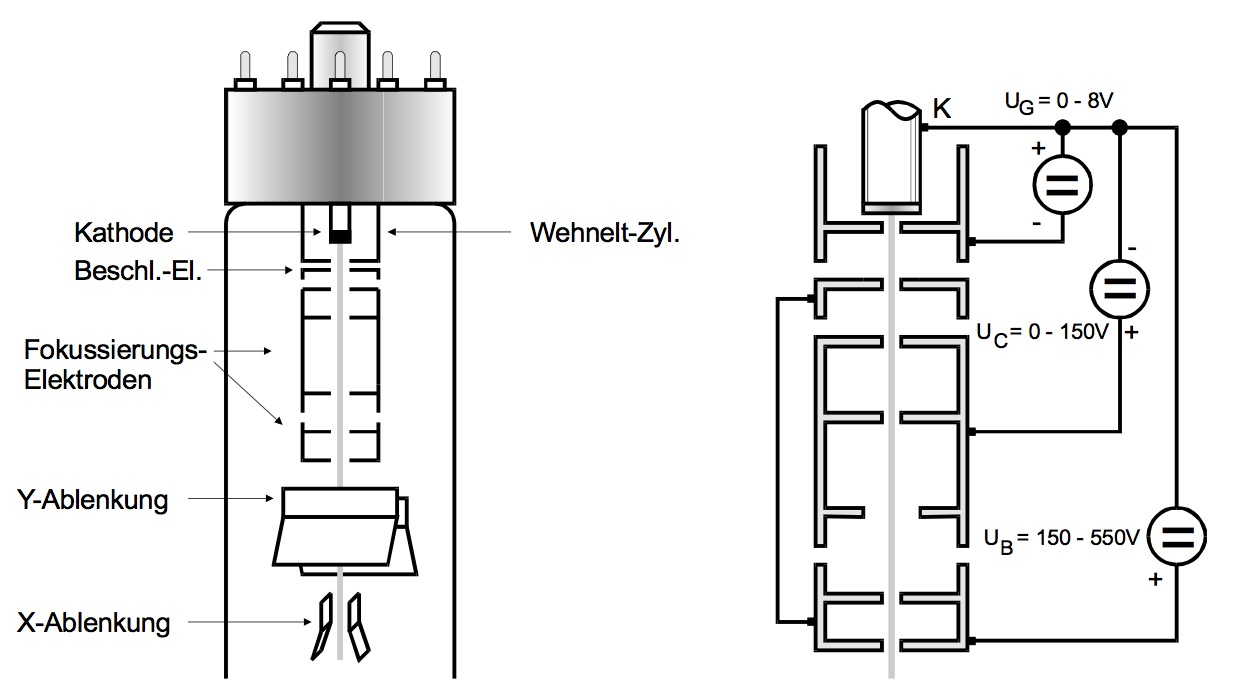
\includegraphics[width = 14cm]{img/wehnelt-z.jpg}
			\caption{Schematischer Aufbau der Braunschen R"ohre -- der Leuchtschirm ist hier nicht sichtbar}
			\label{ablenkung}
		\end{figure}

		\subsubsection{Wehnelt-Zylinder}
		\label{wehnelt}

			Zun"achst wird ein Elektronenstrahl erzeugt. Hierf"ur heizt ein stromdurchflossener Draht einen Zylinder aus einem Material mit geringer Elektronenaustrittsarbeit auf.
			Durch Gl"uhemission treten bei gen"ugend gro"ser Temperatur Elektronen aus.
			Der Zylinder ist von dem gr"o"seren Wehnelt-Zylinder umgeben und es liegt eine Spannung an, sodass der innere Zylinder positiv und der "au"sere negativ geladen ist.
			Durch eine kleine "Offnung in der Stirnseite des Wehnelt-Zylinders treten gerade die Elektronen aus, die gen"ugend kinetische Energie besitzen, um die Potentialbarriere zu "uberwinden.

			Mit einem weiteren Zylinder, der positiv mit der Spannung $U_\mathrm{B}$ geladen ist, werden die Elektronen anschlie"send beschleunigt,
			wobei $v \ll \mathrm{c}$ ist und somit nicht relativistisch gerechnet werden muss.
			Das Durchlaufen dieser Spannung stellt n"aherungsweise die gesamte kinetische Energie f"ur die Elektronen bereit.

		\subsubsection{Fokkusiervorrichtung}

			Die darauffolgende Anordnung aus positiv geladenen Zylindern dient der Fokussierung des Strahls.
			Das elektrische Feld in diesem Bereich wirkt "ahnlich wie Linsen in der Optik.
			Durch Variation der Spannung $U_\mathrm{C}$ kann der Fokus des Strahls ge"andert werden, sodass dieser auf dem Leuchtschirm scharf ist.

		\subsubsection{Ablenkplatten}

			Vor dem Leuchtschirm befinden sich zwei Kondensatoren, deren Platten senkrecht zu\-ein\-ander stehen. Hierdurch kann der Strahl in die Richtungen x und y abgelenkt werden.

			Der Winkel $\theta$, in dem der Kondensator verlassen wird, wird durch Gleichung \ref{theta} be\-schrie\-ben.

			Indem an eine Achse eine S"agezahnspannung mit variabler Frequenz $\omega_\mathrm{takt}$ angelegt wird, kann hiermit ein einfaches Oszilloskop realisiert werden.
			Das Eingangssignal mit fester Frequenz $\omega_\mathrm{sig}$ muss dann an die andere Achse angelegt werden.
			Durch Anpassen der beiden Frequenz $\omega_\mathrm{takt}$ an $\omega_\mathrm{sig}$ l"asst sich ein stehendes Bild des Eingangssignales erzeugen.

		\subsubsection{Leuchtschirm}

			Der Elektronenstrahl trifft schlie"slich auf einen Schirm mit fluoriszierender Beschichtung.
			Die Elektronen wechselwirken mit denen des Schirms und Photonen werden emittiert. Dadurch k"onnen wir den Aufpunkt des Strahls sehen.

	\subsection{Magnetische Kraft (Lorentzkraft)}

		Die magnetische Kraft $\vec{F}_\mathrm{L}$ wirkt nur auf, zum Magnetfeld $\vec{B}$ senkrecht bewegte La\-dun\-gen $q$:

		\begin{eqnarray}
			\vec{F}_\mathrm{L} & = & q \left( \vec{v} \times \vec{B} \right)
		\end{eqnarray}

		Tritt ein Elektron also in ein homogenes Magnetfeld begibt es sich auf eine Kreisbahn.
		Die Lorenztkraft $\vec{F}_\mathrm{L}$ wirkt dann als Zentripetalkraft.

		\newpage
		
		Ist die St"arke $B$ des Magnetfeldes und die Geschwindigkeit $v_0$ des Elektrons bekannt, l"asst sich der Radius $r$ seiner Kreisbahn messen und es gilt:

		\begin{equation}
			r = \frac{m_e}{e} \frac{v_0}{B}
		\end{equation}
	
		Damit kann man also die spezifische Ladung $e / m_e$ bestimmen.\\

		Durch eine Helmholtz-Spule l"asst sich ein nahezu homogenes Magnetfeld erzeugen.
		Setzt man nun eine Braunsche R"ohre in dieses Magnetfeld l"asst sich der folgende Aufbau gut realisieren.

		\begin{figure}[h]
			\centering
			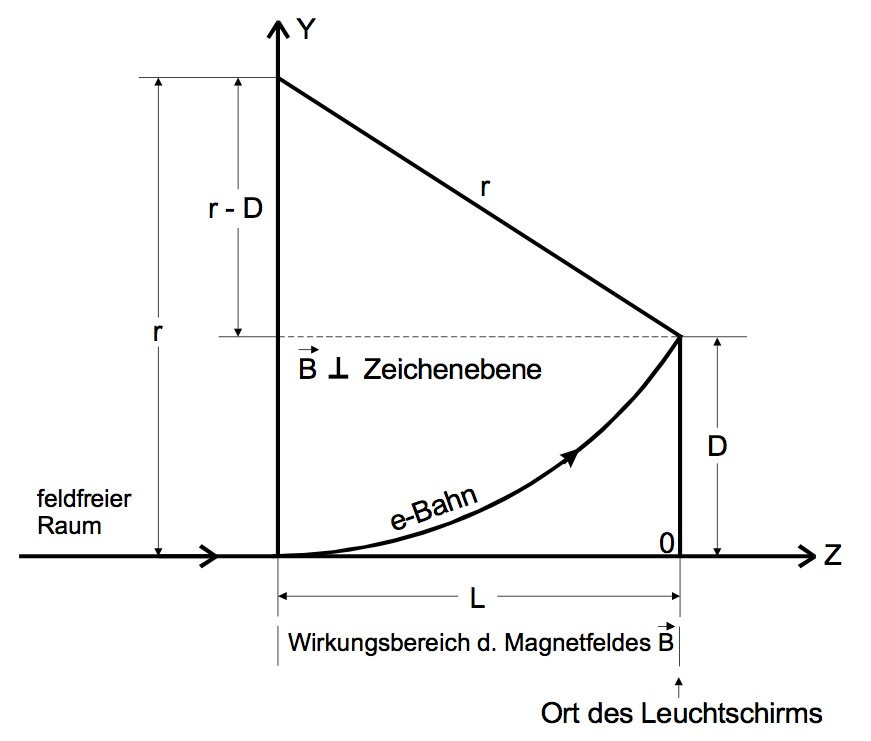
\includegraphics[width = 12cm]{img/magnetfeld.jpg}
			\caption{Strahlablenkung in einem Magnetfeld}
			\label{magnetfeld}
		\end{figure}

		Die Wegl"ange der Elektronen innerhalb der Ablenkkondensatoren der Braunschen R"ohre kann dabei vernachl"assigt werden.
		Die Strecke $L$ ist somit der Weg zwischen Ab\-lenk\-plat\-ten und Leuchtschirm.
		Das Magnetfeld $B$ ist proportional zum Strom $I$ durch die Helm\-holtz\-spu\-le.
		Es gilt dann:

		\begin{equation}
			\sqrt{\frac{e}{m_e}} = \frac{\sqrt{8 U_\mathrm{B}}}{B} \frac{D}{L^2 + D^2}
		\end{equation}


	\newpage

	\section{Aufbau und Durchf"uhrung}
	\label{sec:durchfueuhrung}
	F"ur den Versuch stand ein He-Ne-Laser, ein gr"o"senverstellbarer Einfachspalt , ein gr"o"senverstellbarer Doppelspalt, ein lichtempfindlicher Detektor auf einer mechanischen Schiene sowie ein Amperemeter zur verf"ugung.

	\subsection{Messaufgaben}
		\begin{enumerate}
			\item \label{aufg_1} Punktweises Ausmessen der Beugungsfigur des Einfachspalts (50 Messpunkte). Anschlie"sendes bestimmen der Spaltbreite $b$ und ausmessens der Spaltbreite $b$ mit dem Mikroskop.

			\item \label{aufg_2} Wie \ref{aufg_1} aber mit variablem Einfachspalt und ohne Mikroskop. 

			\item \label{aufg_3} Wie \ref{aufg_1} aber mit festem Doppelspalt und anschlie"sendem Vergleich mit der theoretischen Verteilung des Einfachspaltes.
		\end{enumerate}

	\subsection{Durchf"uhrung}
		\label{sec:durchfuehrung}
		\subsubsection{Messungen}
			\label{sec:messung}

			Der Laser beleuchtet mit einer Wellenl"ange von $\lambda = \SI{633}{\nano \meter}$ wie in \ref{Versuchsaufbau} beschrieben einen ca. $20 - 200 \SI{}{\micro \meter}$ breiten Parallelspalt. Ein lichtempfindlicher Detektor befindet sich in etwa $100 - 120 \SI{}{\centi \meter}$ entfernung vom Spalt, welcher senkrecht zur optischen Achse verstellbar ist.

			\begin{figure}[h]
					\centering
					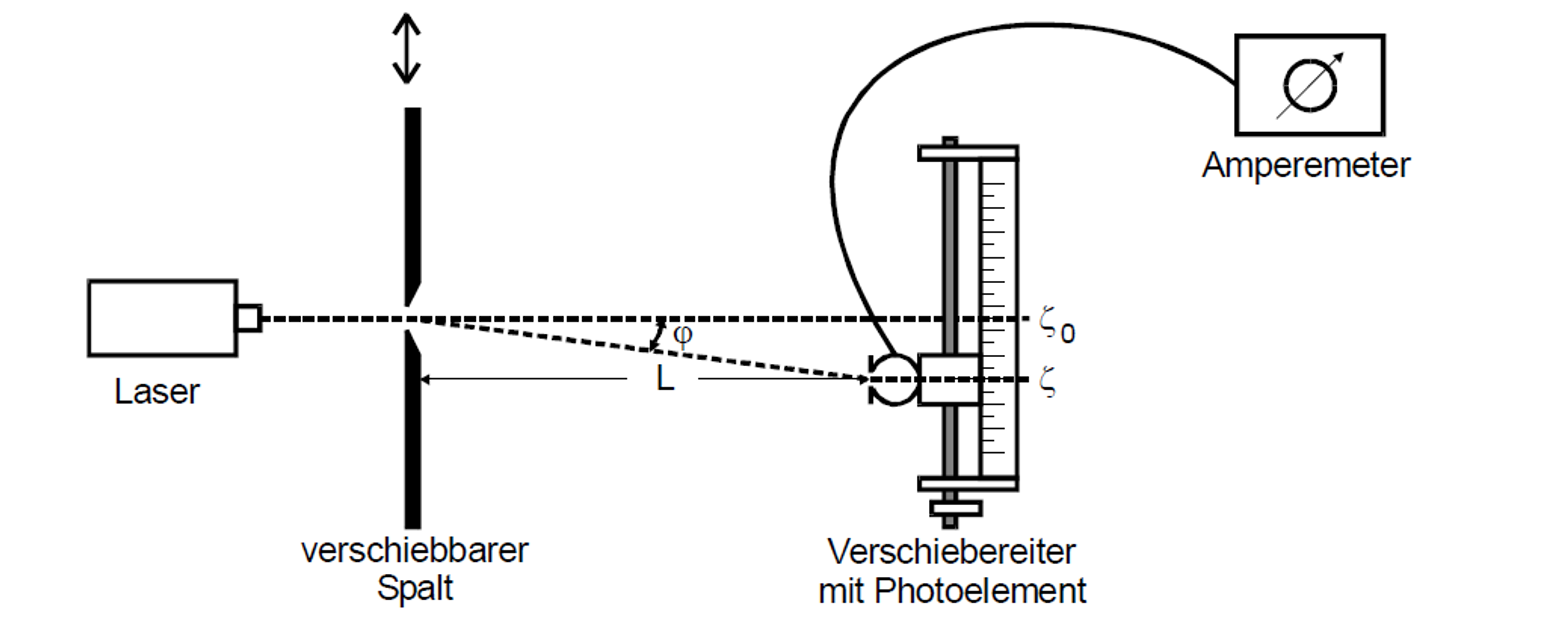
\includegraphics[width = 14cm]{Versuchsaufbau.png}
					\caption{Abb.?}
					\label{Versuchsaufbau}
			\end{figure}

			Anfangs muss die Apparatur justiert werden. Daf"ur wird der Laser fixiert und die h"ohe des Detektors in Mittelstellung so ausgerichtet, dass der Laserstrahl genau auf den Sensor trifft. Anschlie"send wird der f"ur die Messung ben"otigte Spalt in die daf"ur vorgesehene Vorrichtung gesteckt und so daran gedreht bis das Hauptmaximum mittig vom Sensor erfasst wird und die n-ten Nebenmaxima links und rechts des Hauptmaximas in etwa die gleiche Intensit"at haben.

			Nun kann die Intensit"at der Beugungsfigur abh"angig von der Detektorstellung gemessen werden. Dabei wird "uber einen Verschiebeweg von $\SI{50}{\milli\meter}$ die Intensit"at punktweise gemessen. Die genaue Position kann an der Skala der Schiene abgelesen werden. Ein Strich entspricht einem $\SI{}{\centi \meter}$, genauso wie eine Trommelumdrehung. Auf der Trommel kommt eine Skala hinzu, welche in $\SI{}{\micro \meter}$ ablesbar ist.

			Aus der Position des Detektors l"asst sich der Beugungswinkel $\varphi$ aus der Detektorstellung $\zeta$ bestimmen. Dies ist notwendig um die aufgenommene Intensit"atskurve $I(\zeta)$ mit der dem nach ?????? berechneten Verlauf $I(\varphi)$ vergleichen zu k"onnen.

			Es gilt:

			\begin{equation}
				\varphi \approx \tan{\varphi} = \frac{\zeta - \zeta_0}{L}
			\end{equation}

			Dabei ist $\zeta_0$ die Detektorstellung f"ur den ungebeugten Strahl und $L$ der Abstand des Spalts zur Detektoblende.

			F"ur den Doppelspalt wird genauso vorgegangen.

			Zu beachten ist, dass auch bei abgeschaltetem Laser bereits ein sogenannter Dunkelstrom $I_{\text{du}}$ flie"st, welcher daher bei abgedeckter Detektorblende gemessen werden muss.

		\subsubsection{Messung des Abstands per Mikroskop}
			\label{sec:messung_mikro}

			Zun"achst muss das Mikroskop geeicht werden, damit die Breite $b$ des Spalts ausgemessen werden kann. Dies geschieht mithilfe eines Objektmikrometers. Dies ist eine Glasplatte mit einge"atzter Mikrometerskala. In der Brennebene des Okulars liegt eine Skala mit willk"urlicher Teilung. 

			Nach der Fokussierung auf die Skala das Objektmikrometer k"onnen die Skalen verglichen werden und so die Teilung in $\SI{}{\micro \meter}$ ausgedr"uckt werden.


	\newpage

	\section{Auswertung}
	\label{sec:Auswertung}

	\subsection{Bestimmung des Dunkelstroms}
		\label{sub:bestimmung_des_dunkelstroms}
		
		Um die Messwerte mit der Theorie vergleichen zu k"onnen muss zuerst der Dunkelstrom $I_\mathrm{du}$ gemessen werden.

		Dazu wurde unter Versuchsbedingungen, jedoch mit ausgeschaltetem Laser, eine Messung durchgef"uhrt.

		F"ur den Dunkelstrom ergab sich:

		\begin{equation}
			I_\mathrm{du} = \SI{0.13}{\nano \ampere}
		\end{equation}

		Die Aufgetragenenen Messwerte in den Tabellen sind noch nicht um diesen Wert reduziert.

	\subsection{Bestimmung der Spaltbreite eines festen Einfachspalts}
		\label{sub:bestimmung_der_spaltbreite_eines_festen_einfachspalts}
		
		Im folgenden wird die Spaltbreite eines Einfachspalts auf zwei verschiedene Weisen gemessen. Einmal mit Hilfe des Beugungsmusters und einmal mit Hilfe eines Mikroskops.

		\subsubsection{Bestimmung mit Hilfe des Beugungsmusters}
			\label{sub:Bestimmung_mit_Hilfe_des_Beugungsmusters}

			Wie die Spaltbreite bestimmt wird, wird bereits in Abschnitt \ref{sec:messung} erl"autert. Die bereinigten Messwerte finden sich in Tabelle \ref{tabelle_1} wieder.

			Die gemessene Intensit"at wurde in Grafik \ref{graph1} gegen die Detektorposition aufgetragen und eine Theoriekurve nach Gleichung \eqref{prop_einzelspalt} eingef"ugt um die Kurven vergleichen zu k"onnen.

			Zur Anpassung wurde Gnuplot benutzt.

			Es ergibt sich mithilfe der Formel:

			\begin{equation}
				f(x) = a^2 b^2 \left(\frac{\lambda}{\pi b \sin(\frac{x-x_\mathrm{0}}{d})}\right)^2 \sin^2 \left( \frac{\pi b \sin(\frac{x-x_\mathrm{0}}{d})}{\lambda} \right)
			\end{equation}

			der Wert:

			\begin{equation}
				b = \SI{74.6 (17)}{\micro \meter}
			\end{equation}

			\begin{table}[h]
\begin{center}
\begin{tabular}{c|c|c||c|c|c||c|c|c}
Ub[V] & Ud[V] & D[1/4 in] & Ub[V] & Ud[V] & D[1/4 in] & Ub[V] & Ud[V] & D[1/4 in] \\
\hline
200 & -7,1 & 4 & 250 & -9,3 & 4 & 300 & -11,9 & 4 \\
200 & -3,9 & 3 & 250 & -5,2 & 3 & 300 & -7,1 & 3 \\
200 & -0,1 & 2 & 250 & -0,4 & 2 & 300 & -1,2 & 2 \\
200 & 3,4 & 1 & 250 & 4 & 1 & 300 & 4,3 & 1 \\
200 & 6,9 & 0 & 250 & 8,4 & 0 & 300 & 9,5 & 0 \\
200 & 10,5 & -1 & 250 & 12,6 & -1 & 300 & 14,8 & -1 \\
200 & 13,7 & -2 & 250 & 17,3 & -2 & 300 & 20,4 & -2 \\
200 & 17,4 & -3 & 250 & 21,4 & -3 & 300 & 25,3 & -3 \\
200 & 20,7 & -4 & 250 & 25,4 & -4 & 300 & 30,0 & -4 \\
\end{tabular}
\caption{Messwerte zu Aufgabe a bei verschiedenen Beschleunigungsspannungen}
\label{tabelle_1}
\end{center}
\end{table}

			\begin{figure}[H]
				\centering
				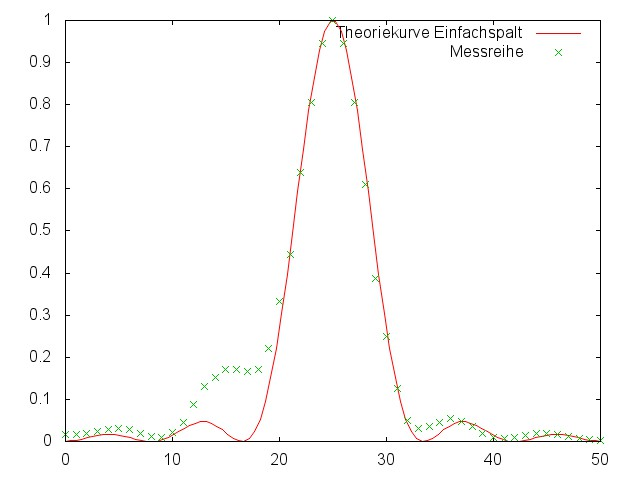
\includegraphics[width = 14cm]{graph1.jpg}
				\caption{Graphische Darstellung der Beugung eines festen Einfachspalt}
				\label{graph1}
			\end{figure}

			Die errechnete Spaltbreite $b$ entspricht nicht exakt der vorgegebenen von $b = \SI{80}{\micro \meter}$. Die Abweichung betr"agt $\SI{6.75}{\percent}$.

			Auf m"ogliche Fehlerquellen wird in der Diskussion eingegangen.
			\newpage

		\subsubsection{Bestimmung mit Hilfe des Mikroskops}
			\label{sub:Bestimmung_mit_Hilfe_des_mikroskops}

			Das Ausmessen mithilfe des Mikroskops wurde bereits in Abschnitt \ref{sec:messung_mikro} erkl"art.
			Es wurde auf das Objektmikrometer fokussiert. Nun wurde der Spalt unter das Objektiv gelegt und mithilfe eines verschiebbaren Teilstrichs die Spaltkanten "uberdeckt. Diese Fixierung wurde dann auf die Mikrometerskala des Objektmikrometers gelegt und ausgemessen.
			Aufgrund von Unsch"arfen wurde ein Fehler von $\sigma_0 = \SI{10}{\micro \meter}$ angenommen.

			Es ergab sich f"ur die Spaltbreite b:

			\begin{equation}
				b = \SI{70}{\micro \meter}
			\end{equation}

			Damit ergibt sich f"ur die gemessene Spaltbreite $b_\mathrm{mikro} = \SI{70 (10)}{\micro \meter}$.
			Es besteht ein Unterschied von $\SI{12.5}{\percent}$ zwischen der gemessenen und der angegebenen Spaltbreite von $b = \SI{80}{\micro \meter}$.
			Auf Fehlerquellen wird in der Diskussion eingegangen.
			\clearpage
			\newpage

	\subsection{Bestimmung der Spaltbreite eines variablen Einfachspalts} 
		\label{sub:bestimmung_der_spaltbreite_eines_variablen_einfachspalts}
		
		Nun sollte die Breite $b$ eines variablen Einfachspalts gemessen werden. Das Messverfahren ist dasselbe wie zuvor.

		Die dazugeh"origen Intensit"atswerte abh"angig von der Detektorposition finden sich in Tabelle \ref{tabelle_2}. Weiter wurde eine Theoriekurve in die Grafik \ref{graph2} einge"ugt, sodass ein Vergleich zwischen Theorie und Experiment m"oglich ist. Daf"ur wurde Gnuplot verwendet.

		Es ergab sich:

		\begin{equation}
			b = \SI{100.0 (23)}{\micro \meter}
		\end{equation}

		\begin{table}[h]	
\centering
\begin{tabular}{|l l||l l||l l|} \hline
	x[mm] & I[nA] & x[mm] & I[nA] & x[mm] & I[nA]\\
	\hline
	0	&	2.5   &  17	&	15  & 34	&	4.8\\
	1	&	2.1   &  18	&	13  & 35	&	3\\
	2	&	2.1   &  19	&	12.5& 36	&	1.85\\
	3	&	2.5   &  20	&	23.5& 37	&	1.55\\
	4	&	2.9   &  21	&	50  & 38	&	2.1 \\
	5	&	2.85  &  22	&	98  & 39	&	2.85\\
	6	&	2.5   &  23	&	135 & 40	&	3\\
	7	&	2.75  &  24	&	165 & 41	&	2.8\\
	8	&	4     &  25	&	155 & 42	&	1.95\\
	9	&	6.2   &  26	&	125 & 43	&	1\\
	10	&	8     &  27	&	92  & 44	&	0.6\\
	11	&	7.9   &  28	&	50  & 45	&	0.51\\
	12	&	6     &  29	&	25.5& 46	&	0.72\\
	13	&	4     &  30	&	11  & 47	&	0.86\\
	14	&	4.8   &  31	&	7.2 & 48	&	0.86\\
	15	&	8.5   &  32	&	6.4 & 49	&	0.68\\
	16	&	13    &  33	&	6   & 50	&	0.45\\
	\hline
\end{tabular}
\caption{Intensit"at des festen Einfachspalts abgh"angig von der Detektorstellung x}
\label{tabelle_2}
\end{table}



		\begin{figure}[H]
			\centering
			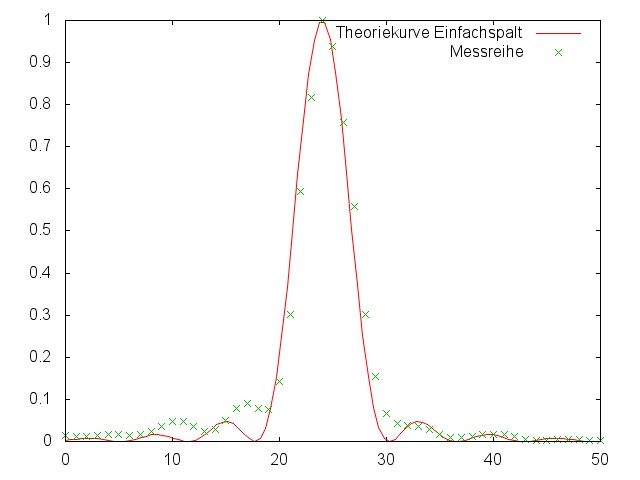
\includegraphics[width = 14cm]{graph2.jpg}
			\caption{Graphische Darstellung der Beugung eines variablen Einfachspalt}
			\label{graph2}
		\end{figure}

		F"ur die Spaltbreite $b$ hat sich in der Messung ein Wert innerhalb des Bereiches von $20-200 \SI{}{\micro \meter}$ ergeben. Da es sich um einen variablen Einfachspalt mit unbekannter Gr"o"se handelt, kann nicht genau gesagt werden wie weit vom tats"achlichen Wert abgewichen wurde. Es ist jedoch mit einem Fehler zu rechnen.

\clearpage
		\newpage
		\newpage
	\subsection{Bestimmung der Spaltbreite eines festen Doppelspalts} 
	\label{sub:bestimmung_der_spaltbreite_eines_festen_doppelspalts}
	
		Auch hier wurde dasselbe Verfahren wie bei den vorherigen Messungen angewendet.
		Die Messwerte sind in Tabelle \ref{tabelle_3} zu finden und der dazugeh"orige Graph mit Theorikurve nach Gleichung \eqref{prop_doppelspalt} in Grafik \ref{graph3}.

		F"ur die Spaltbreite $b$ und den Abstand zwischen den Spalten $d$ ergab sich:

		\begin{eqnarray*}
			b &=& \SI{33.5 (16)}{\micro \meter}\\
			d &=& \SI{226.7 (23)}{\micro \meter}
		\end{eqnarray*}

		Die gemessenen Werte weichen um $\Delta b = \SI{16.25}{\percent}$ und $\Delta d = \SI{9.32}{\percent}$ von den ablesbaren Werten auf der Messscheibe $b = \SI{40}{\micro \meter}$ und $d = \SI{250}{\micro \meter}$ ab.
		M"ogliche Fehlerquellen kommen in der Diskussion.

		\begin{table}[h]	
\centering
\begin{tabular}{|l l||l l||l l|} \hline
	x[mm] & I[nA] & x[mm] & I[nA] & x[mm] & I[nA]\\
	\hline
	0	&	1     &  17	&	6.4   & 34	&	2.8\\
	1	&	2.3   &  18	&	25    & 35	&	10\\
	2	&	1.6   &  19	&	8     & 36  &	2.8\\
	3	&	1.4   &  20	&	26    & 37  &	3.4\\
	4	&	0.98  &  21	&	24    & 38	&	2.9\\
	5	&	0.6   &  22	&	12.5  & 39	&	0.66\\
	6	&	0.78  &  23	&	38    & 40	&	1.25\\
	7	&	0.36  &  24	&	9.4   & 41	&	0.38\\
	8	&	0.58  &  25	&	32    & 42	&	0.34\\
	9	&	0.53  &  26	&	22.5  & 43	&	0.36\\
	10	&	1.25  &  27	&	17    & 44	&	0.3\\
	11	&	2.25  &  28	&	32    & 45	&	0.5\\
	12	&	1.6   &  29	&	6.8   & 46	&	0.5\\
	13	&	7     &  30	&	28    & 47	&	0.68\\
	14	&	3.2   &  31	&	10.5  & 48	&	0.68\\
	15	&	9.6   &  32	&	10.5  & 49	&	0.64\\
	16	&	12.5  &  33	&	16    & 50	&	0.77\\
	\hline
\end{tabular}
\caption{Intensit"at des festen Doppelspalts abgh"angig von der Detektorstellung x}
\label{tabelle_3}
\end{table}



		\begin{figure}[H]
			\centering
			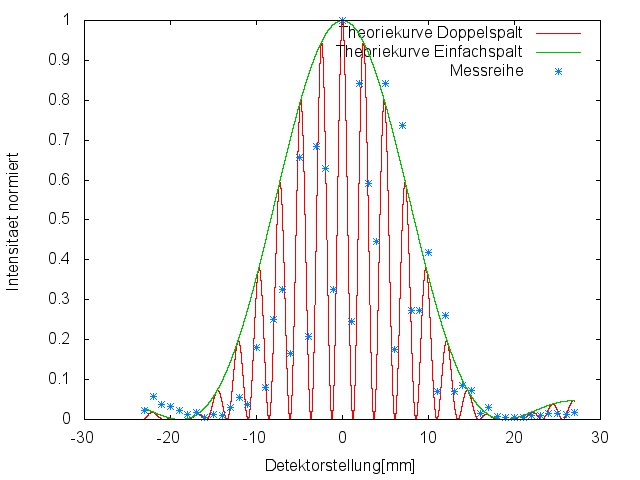
\includegraphics[width = 14cm]{graph3.jpg}
			\caption{Graphische Darstellung der Beugung eines festen Doppelspalts}
			\label{graph3}
		\end{figure}
		\clearpage


	\newpage

	\section{Diskussion}
	\label{sec:diskussion}

	Allgemein l"asst sich sagen, dass sich die theoretisch hergeleiteten Beziehungen besonders gut in den ersten beiden Messreihen wiedergespiegelt haben.
	Die Auswertung dieser Daten lieferte Werte f"ur Spaltbreite und -abstand, die sehr nahe an den Herstellerangaben lagen.

	Die dritte Messreihe lieferte auf den ersten Blick "au"serst diffuse Werte. Dies lag an der geringen Aufl"osung der Messpunkte.
	Mit mehr Messpunkte h"atte ein Fit hier genauere Werte f"ur Spaltbreite- und abstand des Doppelspaltes liefern k"onnen. Dennoch waren die so gewonnenen Werte durchaus akzeptabel.\\

	Die Fehlerquellen waren bei allen Messungen jedoch sehr gro"s.
	Die zuvor gemessene Dunkelspannung $I_\mathrm{du}$ hat h"ochst empfindlich auf Ver"anderungen der Lichtverh"altnisse im Laborraum reagiert.
	Durch Ein- und Ausschalten der Lampen an anderen Versuchstischen oder das "offnen der Eingangst"ur konnten die Messwerte somit leicht beeintr"achtigt werden.
	Zudem stellte das Justieren der Versuchsapparatur eine gro"se Fehlerquelle dar.
	Der Laser konnte lediglich durch eine Stellschraube in H"ohe und Ausrichtung fixiert werden.
	So war es schwierig, die Photozelle exakt zu treffen.
	Ebenso konnte nicht ausgeschlossen werden, dass die Photozelle genau senkrecht zum Laser zeigte.
	Dadurch traf auf einer Seite eventuell mehr licht frontal auf die Zelle, als auf der anderen.
	Dies w"urde den Intensit"atsunterschied neben dem Hauptmaximum in unseren Messdaten erkl"aren.\\
	
	Schlie"slich l"asst sich "uber die Messung der Spaltbreite mit dem Mikroskop nur sagen, dass diese Methode "au"serst ungenau ist.
	Zwar war das Ergebnis in derselben Gr"osenordnung wie die Herstellerangabe, die Empfindlichkeit der Optik war jedoch so gro"s, dass wir die Aussagekraft dieser Messung stark bezweifeln.
	Die geringe Tiefensch"arfe des Mikroskopes machte eine genaue justierung auf die R"ander des Spaltes sehr schwierig.

\section{Literatur}

	Alle Grafiken wurden eigenst"andig mit Gnuplot oder pyplot erstellt oder aus der Versuchsanleitung \"Beugung am Spalt\" der TU Dortmund (Stand 29.10.12) entnommen.

	%\anhang

\end{document}